% !TEX root = main.tex

\section{Experiments} \label{sec:experiments}

We use the dataset made available thanks to Angermann et. al. \cite{angermann2010high} to validate our method and compare the results to provided outputs from the state-of-the-art Kalman filter.
Our method is applied on several scenarios from these dataset and we present typical results obtained with two representative cases. The first sets of data correspond to a human walking back and forth 
while the second example is related to a walking pattern describing a eight-shape. Both IMU and motion capture data are provided at 100 Hz.

Then, we will investigate the use of additional sensors to demonstrate the feasibility of fusion strategies using a low cost IMU running at 1 kHz (Invensense's MPU6050~\cite{InvenSense}).

% We use a low-cost IMU in our application to demonstrate the feasibility of our method. 
% To that end, we selected the MPU6050 from Invensense, which combines triaxial accelerometers and gyrometers, provides 1kHz data rate, and is extensively used in the open source community.

\subsection{Method}

Keyframes are created at the beginning and ending of each support phase of the selected foot according to ZUPT detection provided by the dataset. Factors active in the graph (see \figRef{fig:factor_graph}) are: initial position and yaw; zero velocity, bias drift, and IMU pre-integration. We only use the bias magnitude 
and zero velocity constraint factors in the initial keyframe. All the graph is optimized after each keyframe creation so that these estimates can be used for future estimations with new keyframes. Zero velocity constraints are applied 
as a fixed prior for the optimizer, meaning that corresponding variables will not be estimated but considered as parameters. As a consequence, we need to be confident that timestamps detected as zero velocity instants really match static phases of the IMU. 
Otherwise we would be imposing a constraint inducing a wrong estimate of the trajectory.

In order to show how interesting fusion strategies can be, we simulate the use of an odometry sensor providing the displacement of the foot between two frames at a frequency that is lower than IMU.
This specific case is a common use of IMUs in fusion strategies to reduce the drift error due to IMU's biases \cite{santamaria2015high}. With a better estimation of its biases, the IMU can then be used to detect events related the human wearing the device.
Such strategy can be implemented with RFID sensors or more basically with visual odometry. 
In our case, we use motion capture information to reconstruct odometry between consecutive keyframes, allowing us to create keyframes during the flying phases of the foot. As in the usual ZUPT-aided inertial
navigation, zero-velocity constraints are imposed only on keyframes created during contact phases. Kinematic odometry is also added between all consecutive keyframes (see \figRef{fig:factor_graph}).

%The parameters we need to calibrate for a correct integration are the IMU biases, on top of which we integrate the incoming IMU data.
%The time varying property of the bias is a critical point to consider in order to avoid large deviations. 
%This calibration is made possible
%through the dependencies of the delta pre-integration (${\Dp}(\bfa_b, \bw_b), {\Dv}(\bfa_b, \bw_b), {\Dq}(\bw_b)$). 
%Fusing both odometer and IMU provides constraints on position and orientation parts of
%the state vector. 
%However, velocity is still not observable and is affected by the bias estimation. 
%In the case of legged locomotion, we fix the observability problem by adding a zero velocity constraint when the foot is stable on the ground.
%
%The initial orientation estimation is made possible by adding an absolute constraint on yaw part of the state vector, otherwise we would run into observability problems. \textbf{add figure here (graph)}

\subsection{Results}
\subsubsection{State estimation using ZUPT only}

As motion capture data are not used during the experiments, the system is not provided with enough information to be able to precisely estimate the vertical orientation of the IMU due to its non-observability from the IMU measurements directly. 
As a consequence, the estimation of the state of the foot is not able to converge to its real value. In other words, the foot trajectory can be recovered up to a rotation around the gravity axis. 
In the following, we manually translate the first estimated states to the initial reference one and rotate the estimated trajectories in order to compare our results against the ground-truth measurements.
Our system is able to estimate the state of the system to a precision close to the state-of-the-art 9-state Kalman filter \cite{foxlin2005pedestrian} as shown in \figRef{fig:8shape_walk}.
Results of bias estimation using another dataset provided by the DLR are given in \figRef{fig:curve_walk}.

Besides, the experiment shows satisfying results in terms of computational times. Indeed, 3.1 seconds are enough to integrate all the data corresponding to a 50 seconds experiment, that is more than 5000 IMU data, to build and to optimize the graph each time a keyframe is created with our framework,
with a total of 80 keyframes. It would be hard, if not currently impossible, to get such results using the IMU without a proper pre-integration method.
The optimization part is currently handled by Google Ceres optimizer~\cite{ceres-solver} using the sparse structure of the problem. All in all, it takes $98 \mu s$ in average to read and integrate a single IMU measurement including the computation of jacobians.

\subsubsection{State estimation using ZUPT and sensor fusion}

The strength of the optimal estimation can also be found in the fusion strategies. 
\figRef{fig:forward_walk_IRI} shows the reconstructed foot trajectories for the two cases: without and with the flying keyframe information. Adding kinematic information between keyframes enhances the observability of the system and allows to a better estimation.
A major advantage of IMU's pre-integration theory is the ability to use past pre-integrations corrected with current estimates of keyframes and biases as simply as it takes to integrate a single IMU data. This removes the need of linearization of
intermediate IMU data between previous and current estimates of the state on which the integration must be performed. We also notice that the use of a flying keyframe makes the bias estimation more stable.

% The MOCAP provides more controlled conditions for the kinematic measurements.
% \figRef{fig:forward_walk_IRI} shows the reconstructed foot trajectories for the cases without the flying KF, and with the flying KF. We can observe a correct estimation only when the flying KF is added. Bias autocalibration is also more stable with the flying KF.

% %Then we show that using an IMU on the foot of the robot leads to a better estimation of the real position of the member compared to encoder based odometry. 
% %We check the feasibility of the trajectory reconstruction using a 1Khz IMU attached to one's foot and tracked with a motion capture (MOCAP) system. The MOCAP is used to get odometry between zero-velocity phases, i.e. when the foot is on the ground,
% %and will be taken as the ground truth against which we compare the trajectory reconstruction.
% %
% %We reproduce the movements the feet of a robot could have when it is walking. However, as shown in figures \textbf{add figure here}, the final optimal state
% %is not the expected one and acceleration biases are rapidly changing. The variation that we can see is not only due to some random walk and can be explained by the excitement of biases in a different axis.
% %As explained in \cite{roussillon2011rt}, in opposition to gyroscope biases, acceleration biases do not converge toward stable values during a motion exciting several axis of the sensor. 
% %This effect can be explained by time inconsistency meaning that we fail
% %to use the information of the entire motion to converge toward stable values as expected in the sensor model, but the problem may also be that the step motions do not use all the axis of the accelerometer as it should.

\begin{figure}[tb]
\centering
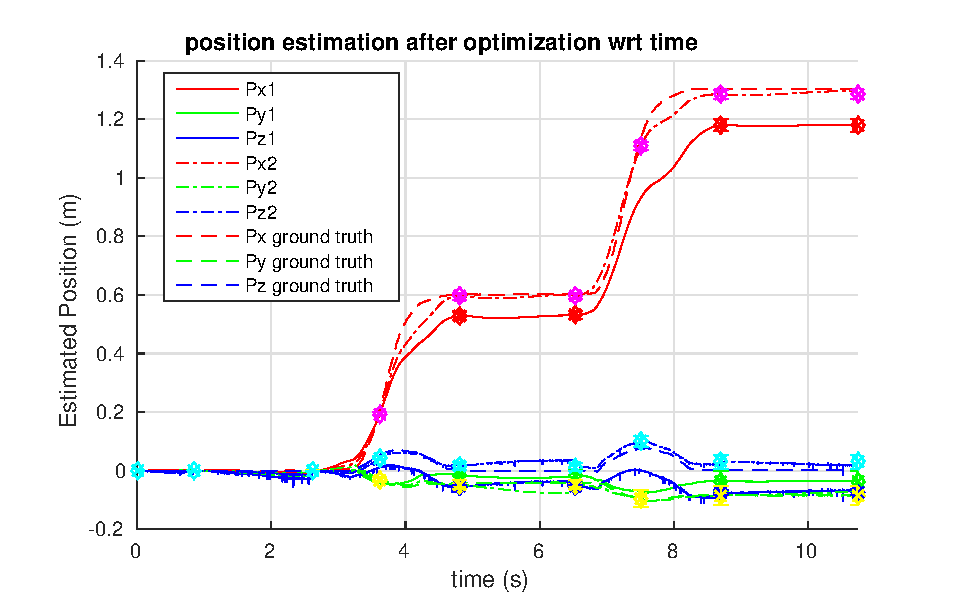
\includegraphics[scale=0.7]{figures/Result_position}
\par\vspace{4mm}
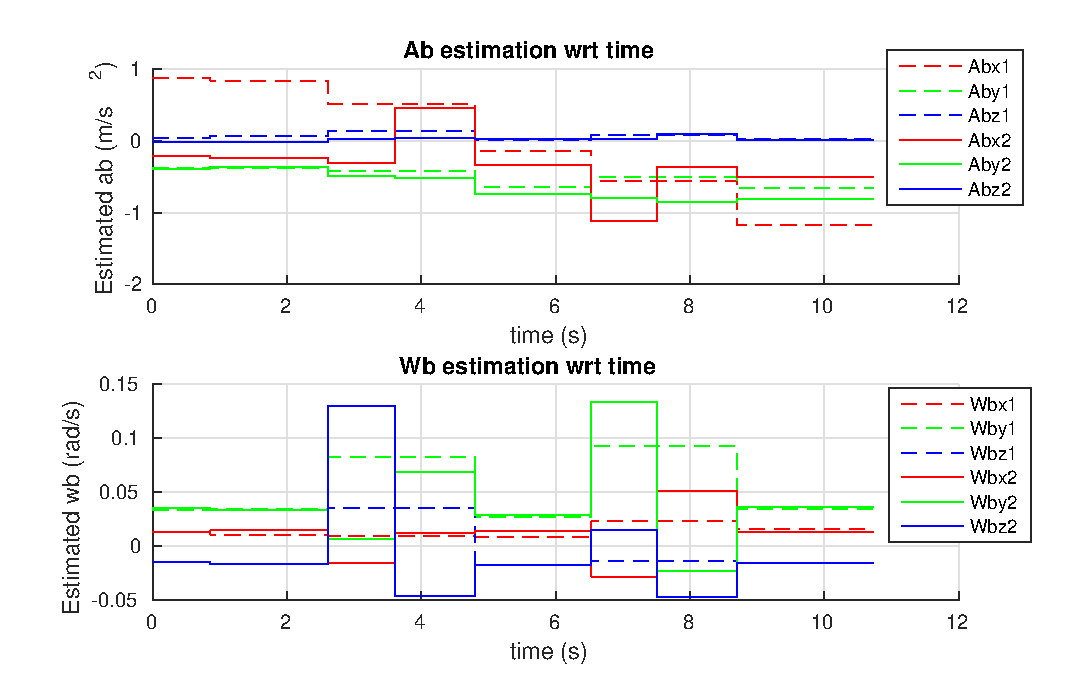
\includegraphics[scale=0.7]{figures/Result_bias}
\caption{ 
{\bf Top}: trajectory estimation during human walking with an IMU attached to a foot. Continuous, dashed and dashed-dot lines are respectively: ground truth, 
estimation with zero velocity constraints only, estimation using zero velocity constraint and 1 odometry measurement during foot's flying phase. Odometry was here built from motion capture data.
{\bf Bottom}: Evolution of corresponding estimated IMU biases 
}
\label{fig:forward_walk_IRI}
\end{figure}

% \begin{figure}[tb]
% \centering
% 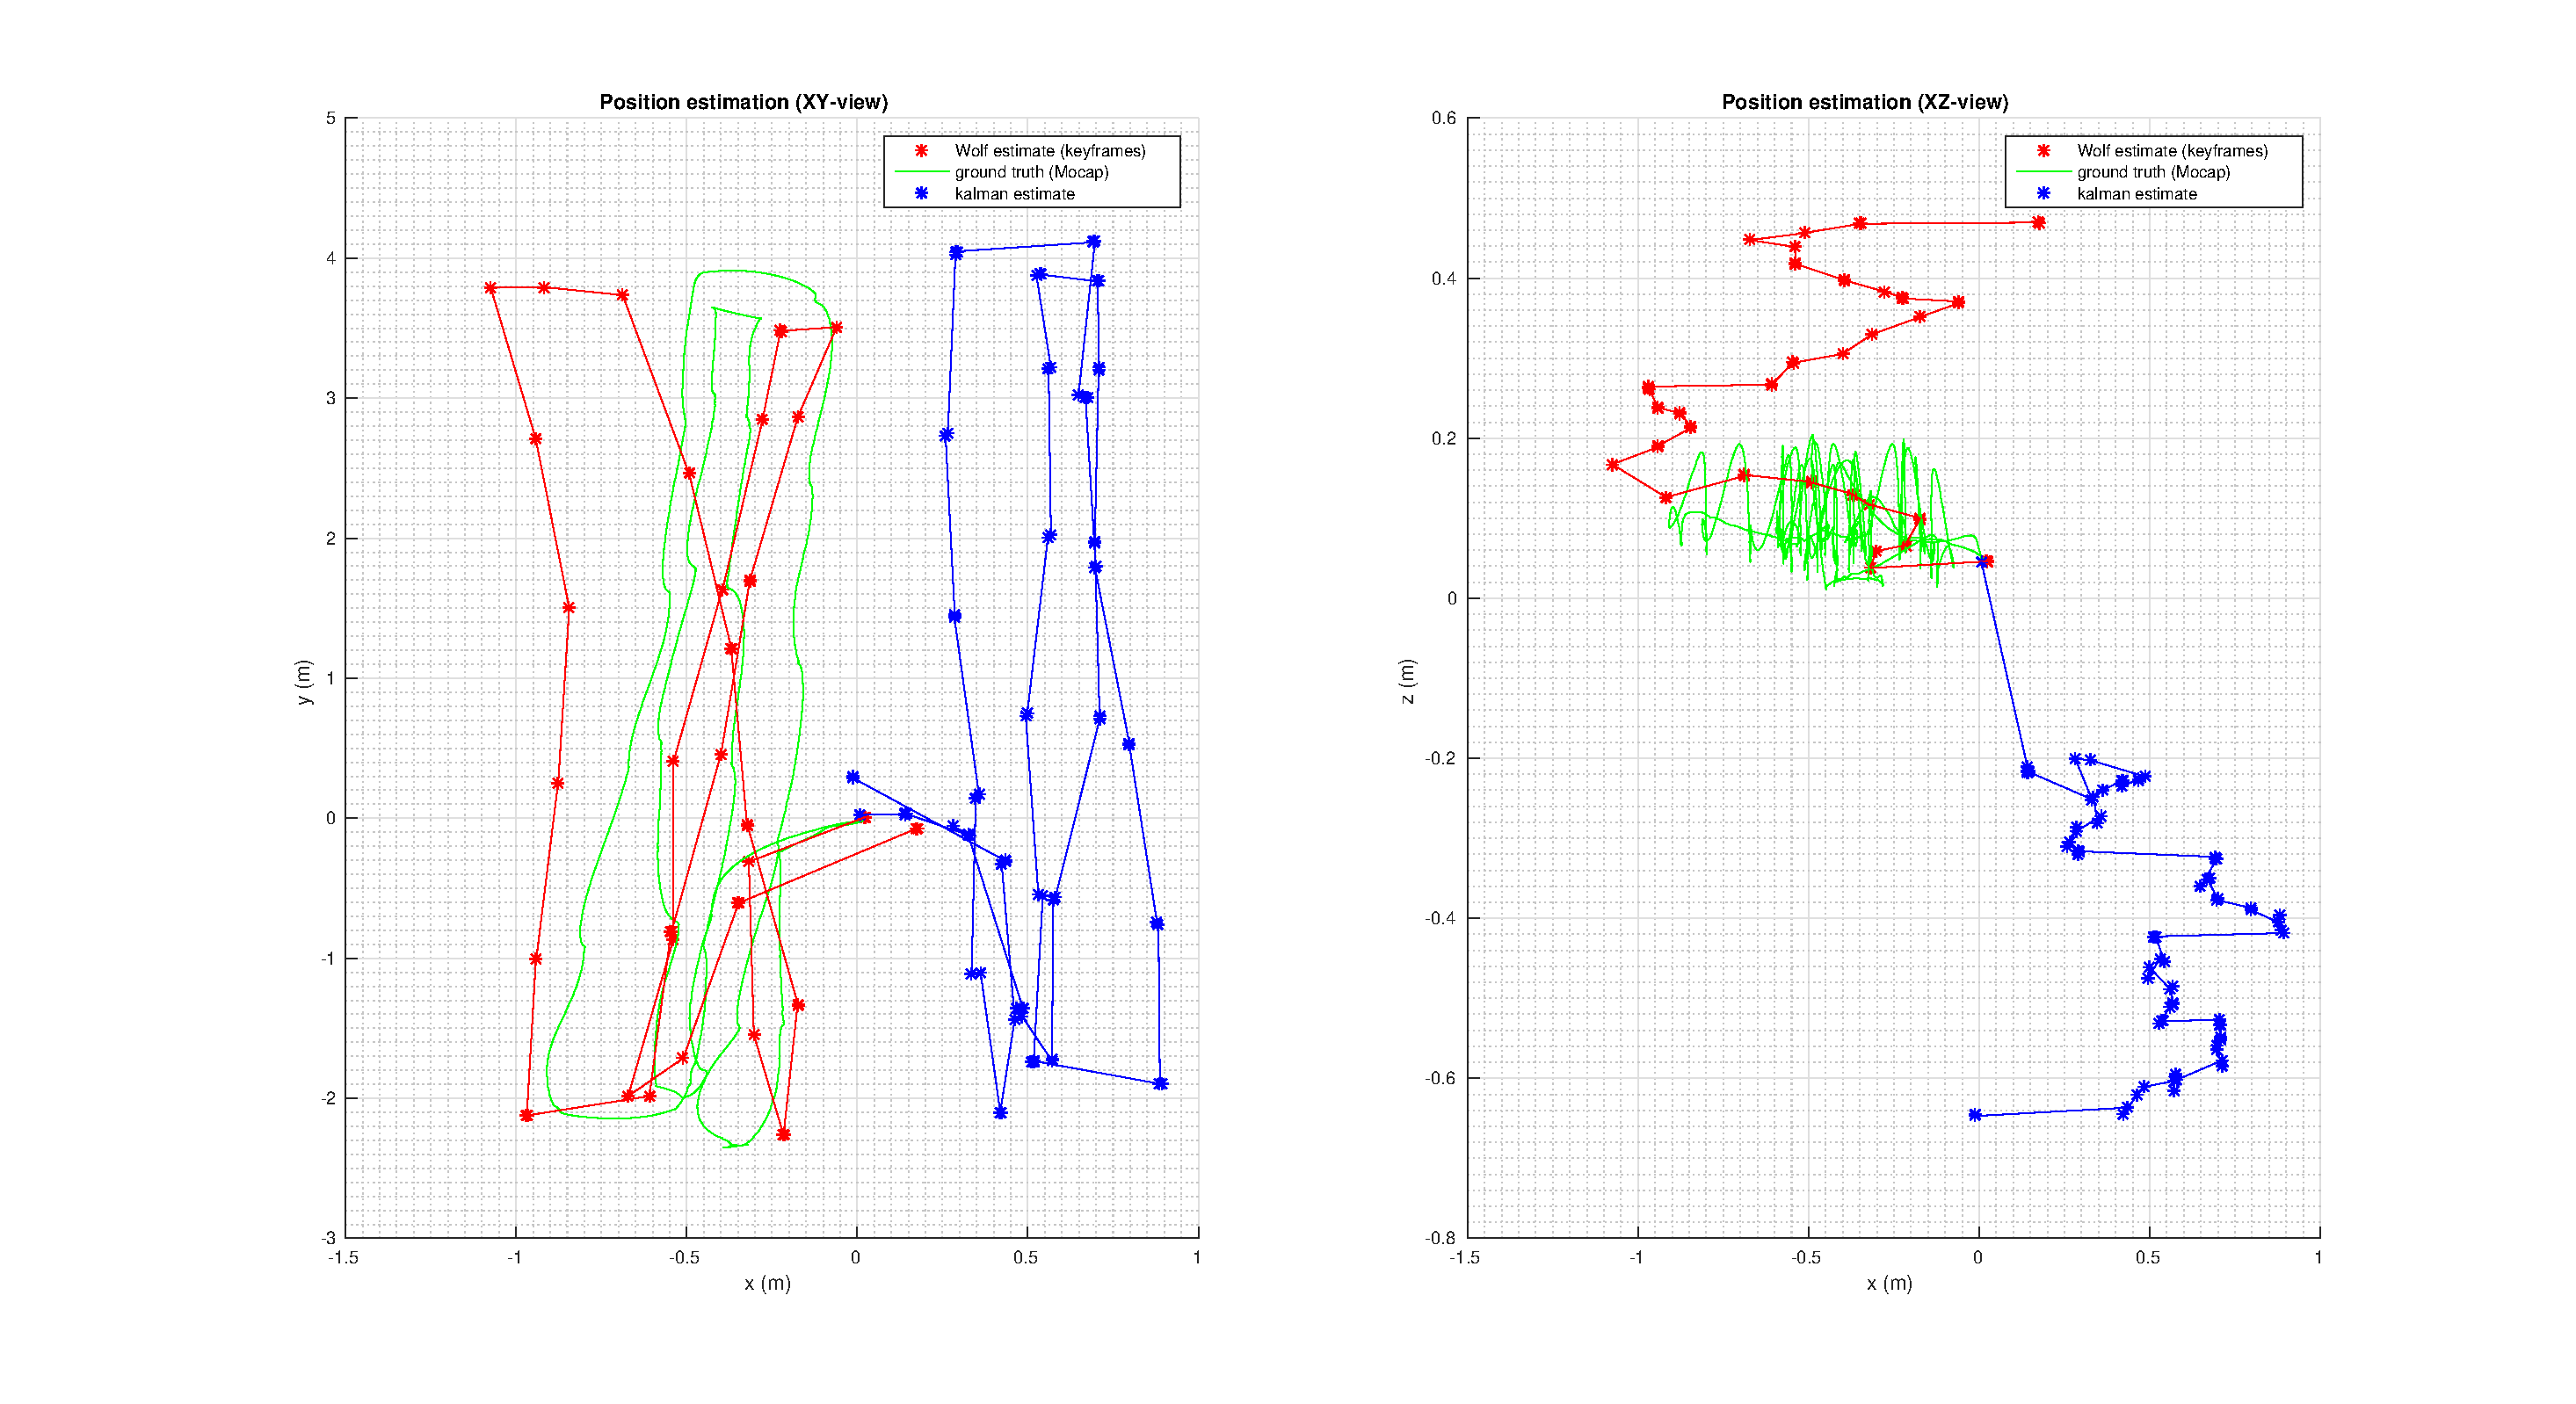
\includegraphics[scale=0.175]{figures/experiments/straight_walk/XY_XZ_viewsRotated.eps}
% \par\vspace{4mm}
% 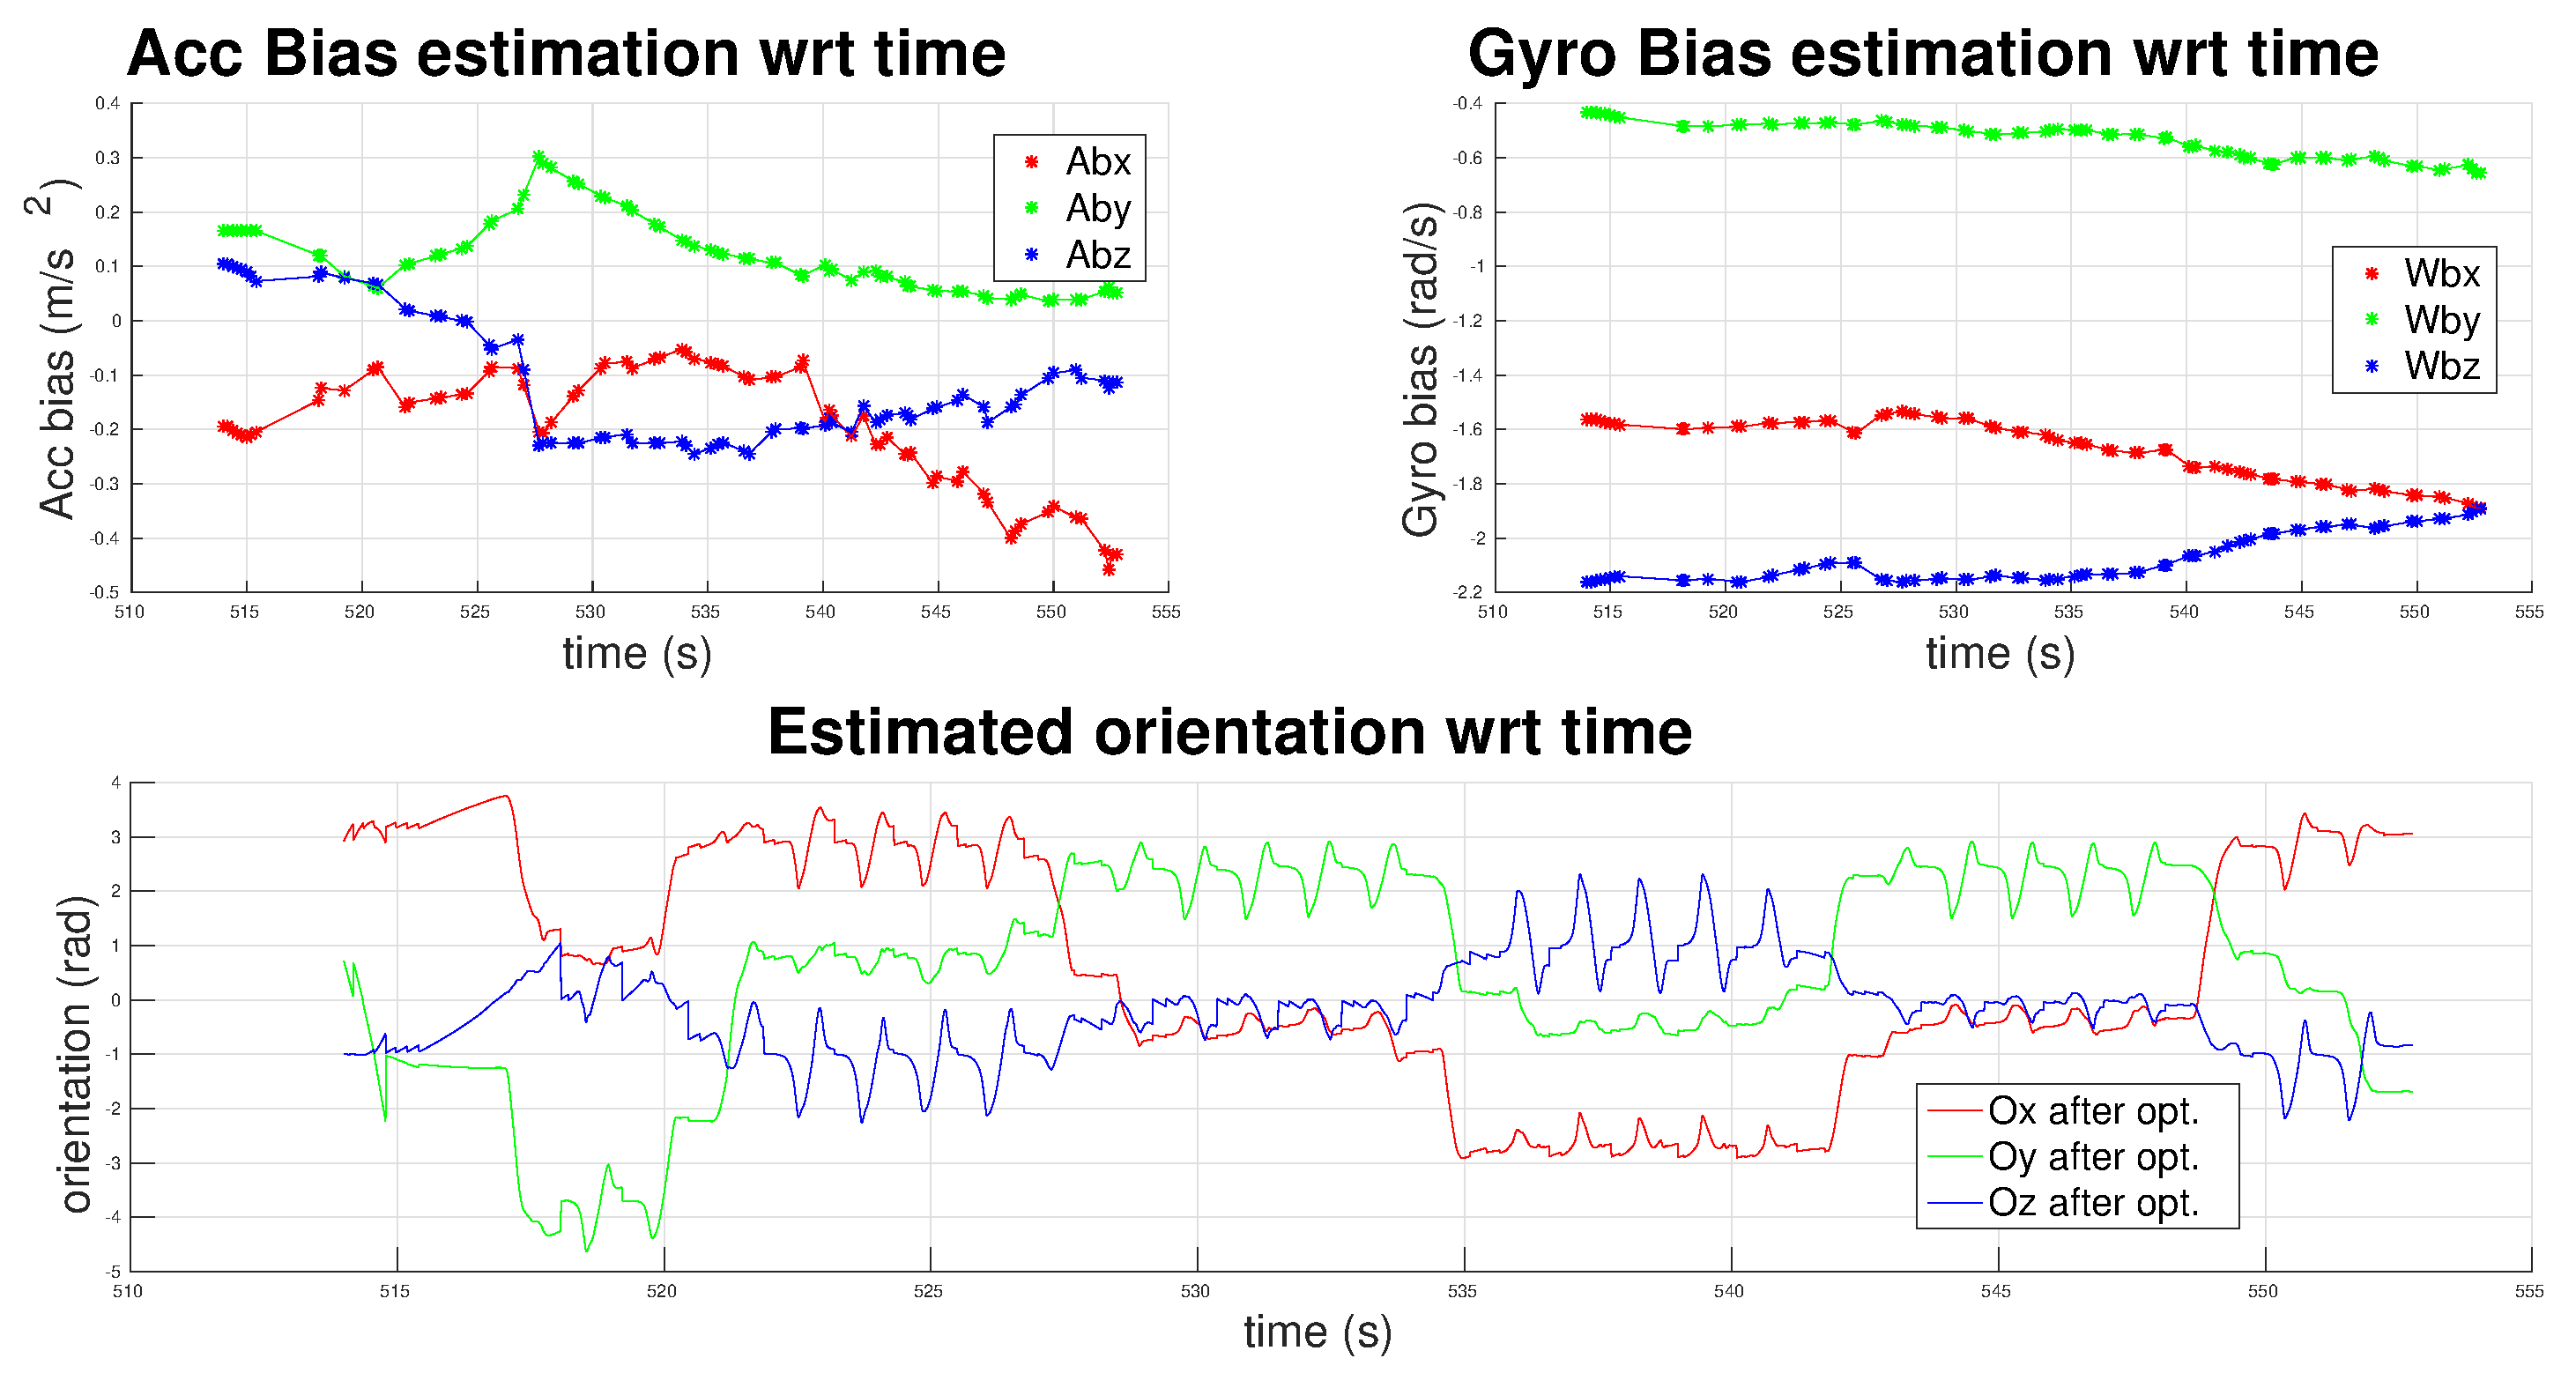
\includegraphics[scale=0.175]{figures/experiments/straight_walk/bias_orientation.eps}
% \caption{ 
% {\bf Top}: trajectory estimation during human walking with an IMU attached to a foot. We used data recorded during straight walk phases. Stars in blue and red colors are respectively the reference estimated states provided in the dataset and the estimation with our approach.
% The continuous green line is the ground truth as given by the motion capture system.
% {\bf Bottom}: Evolution of estimated IMU biases and orientation of the device. Biases are estimated only for keyframes and considered as constant between them. 
% }
% \label{fig:straight_walk}
% \end{figure}

% \begin{figure}[tb]
% \centering
% 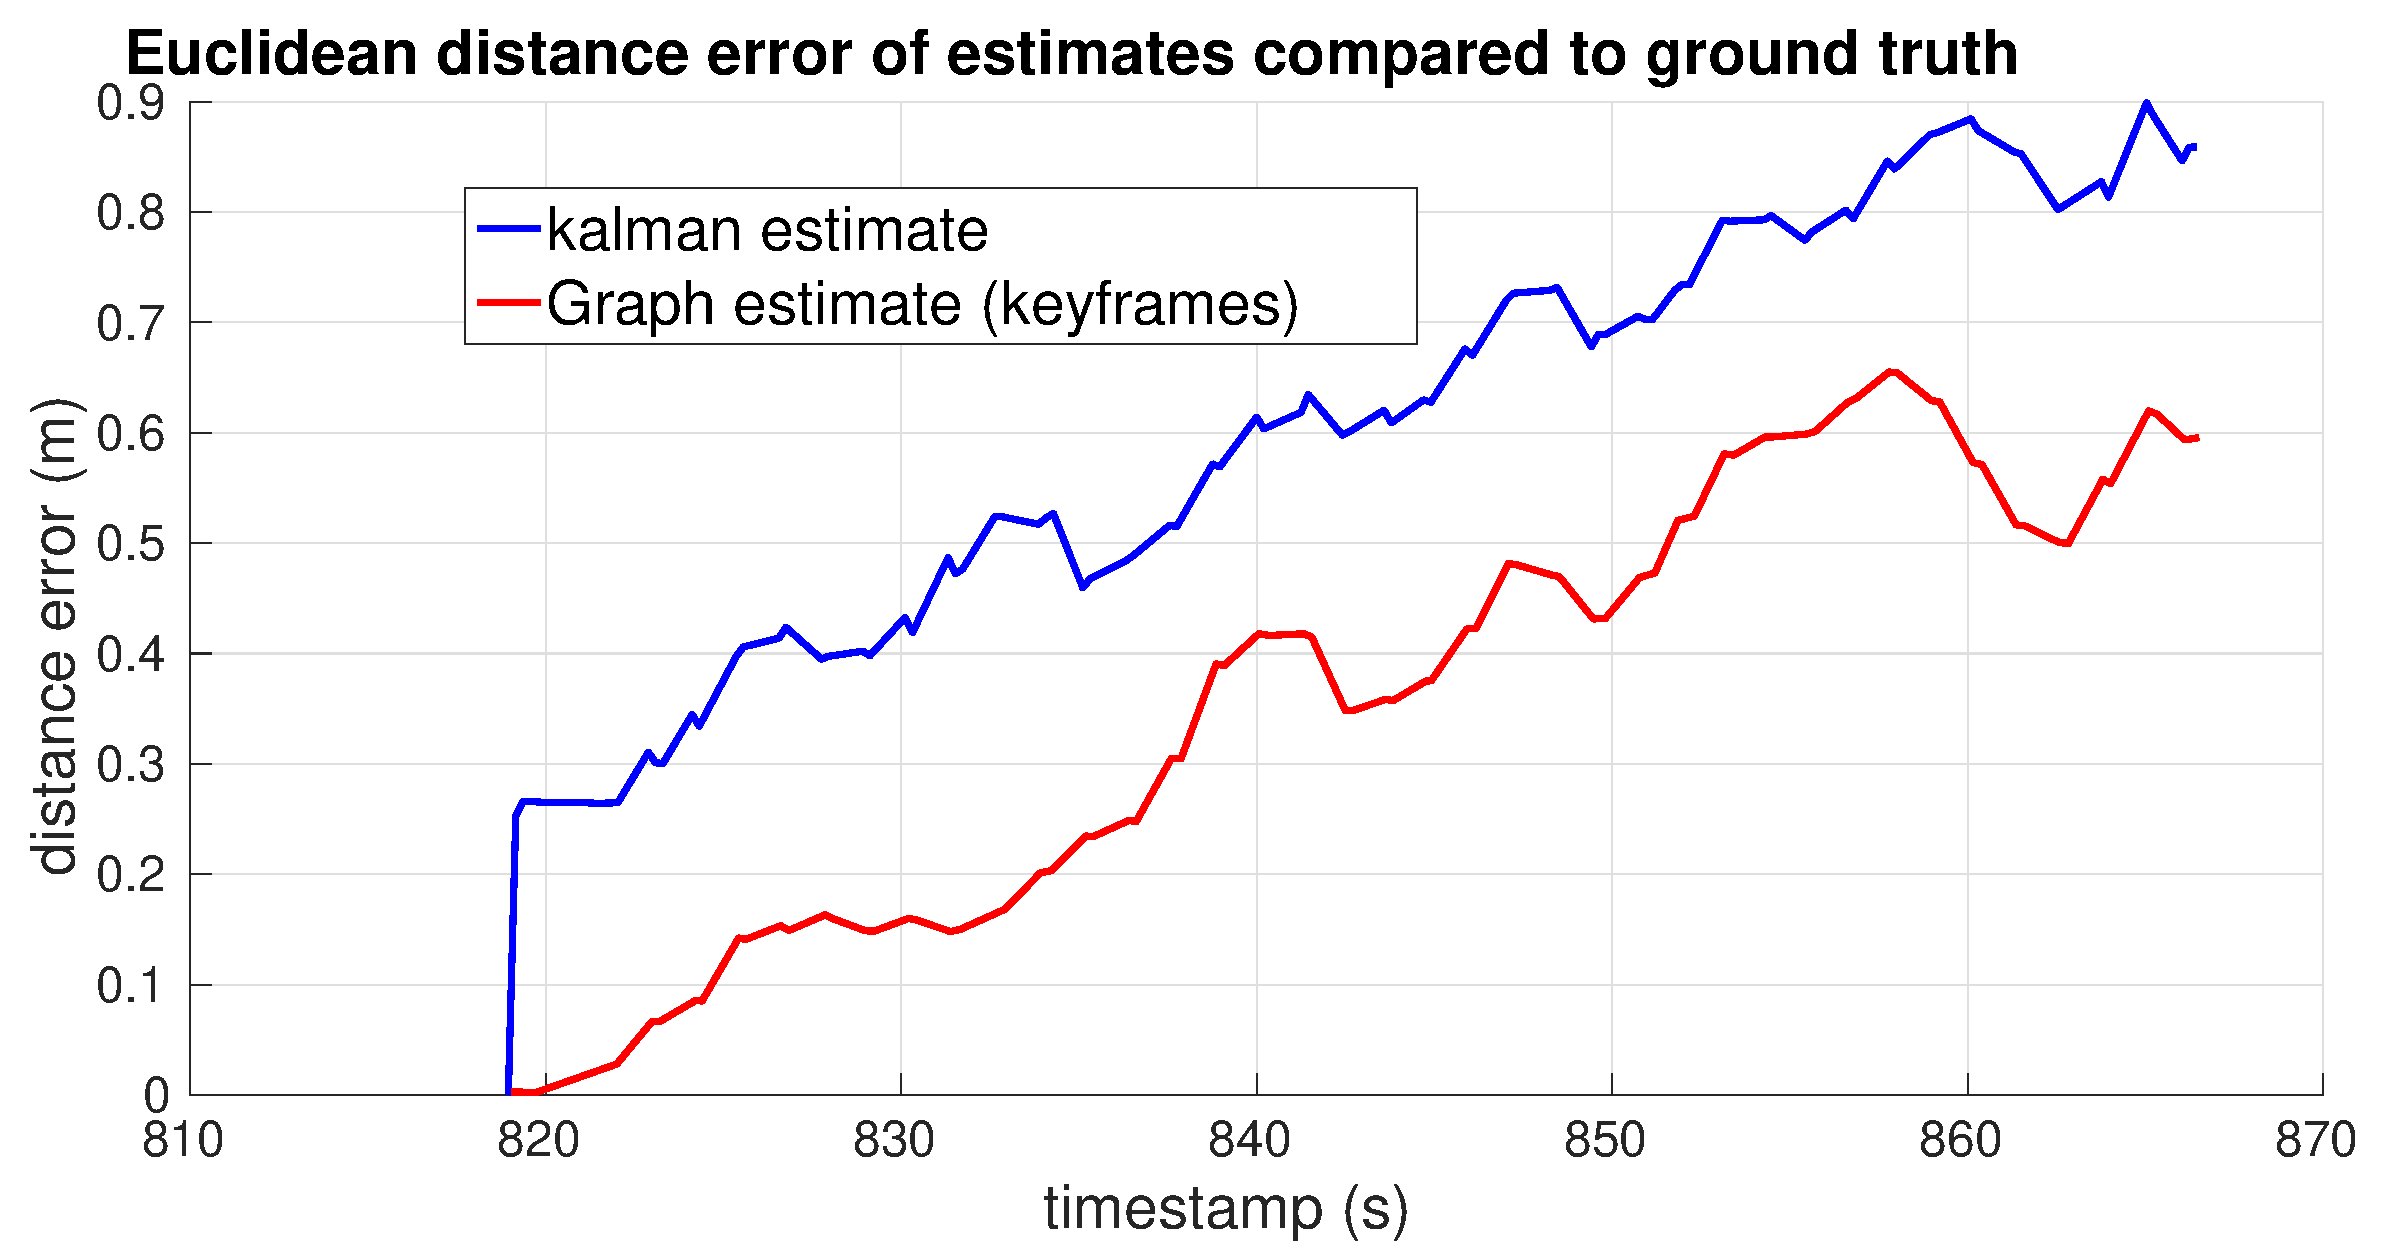
\includegraphics[scale=0.175]{figures/experiments/8shape/euclidean_err.eps}
% \caption{ 
% {\bf Top}: trajectory estimation during human walking with an IMU attached to a foot. We used data recorded during straight walk phases. Stars in blue and red colors are respectively the reference estimated states provided in the dataset and the estimation with our approach.
% The continuous green line is the ground truth as given by the motion capture system.
% {\bf Bottom}: Evolution of estimated IMU biases and orientation of the device. Biases are estimated only for keyframes and considered as constant between them. 
% }
% \label{fig:8shape_walk_err}
% \end{figure}

\begin{figure}[tb]
\centering
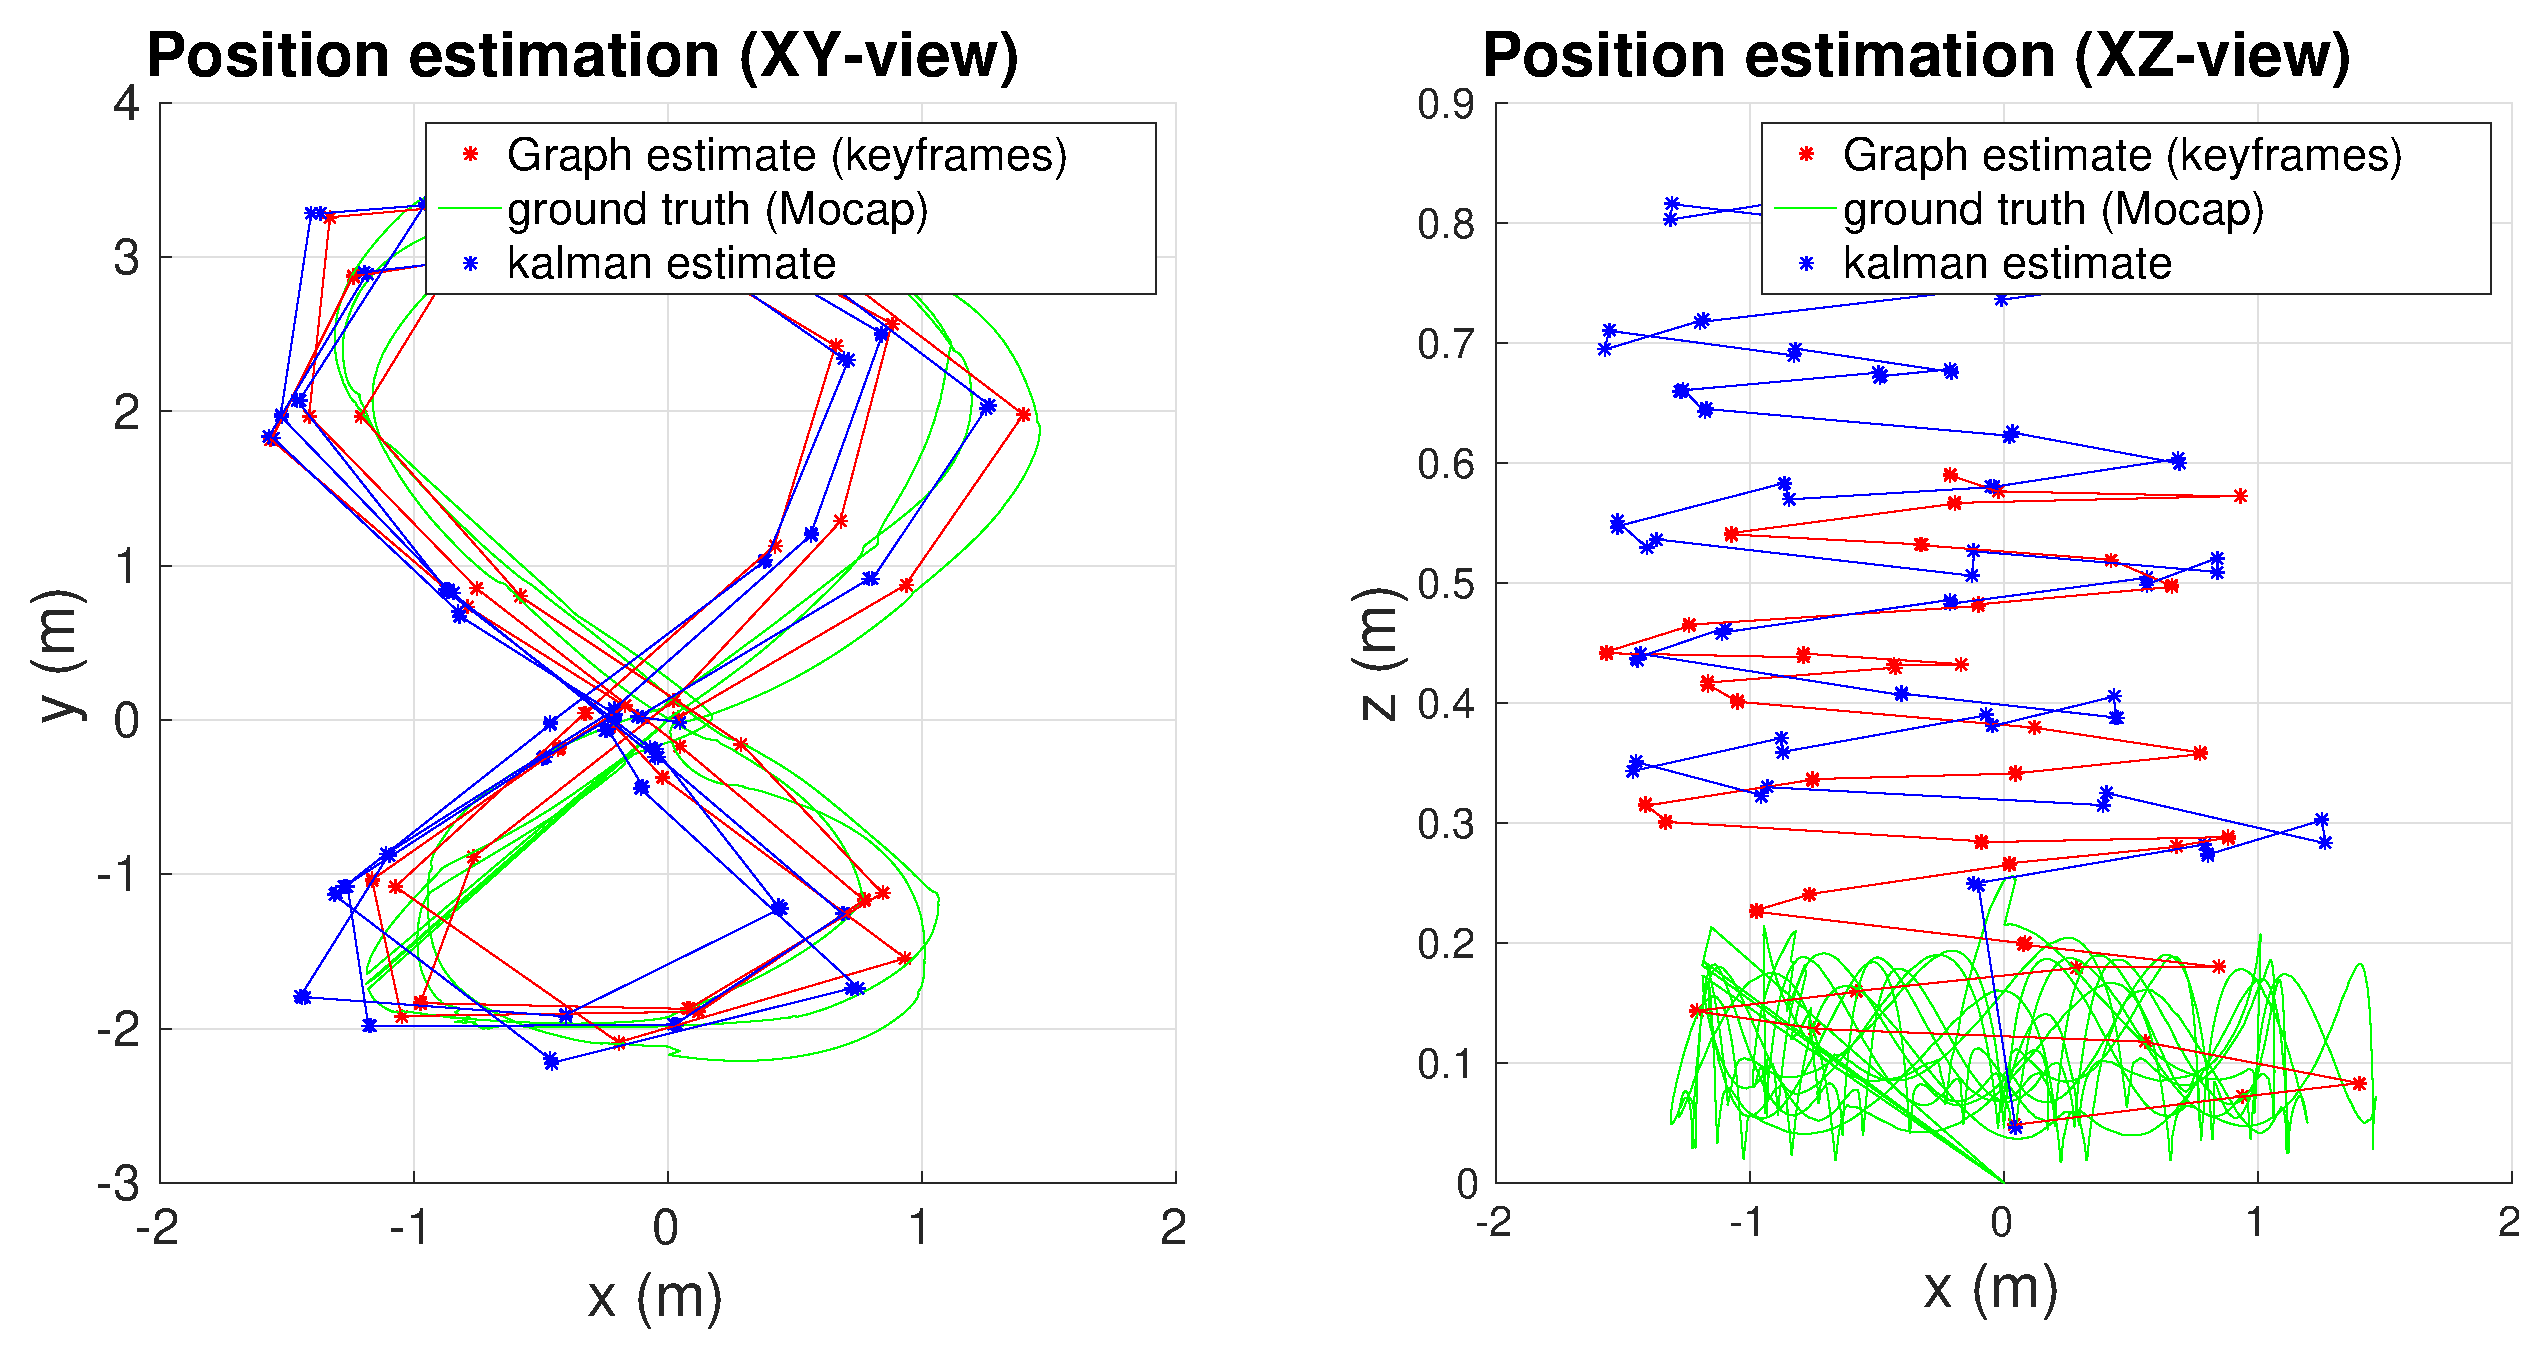
\includegraphics[scale=0.3]{figures/experiments/8shape/XY_XZ_viewsRotated2.eps}
\par\vspace{4mm}
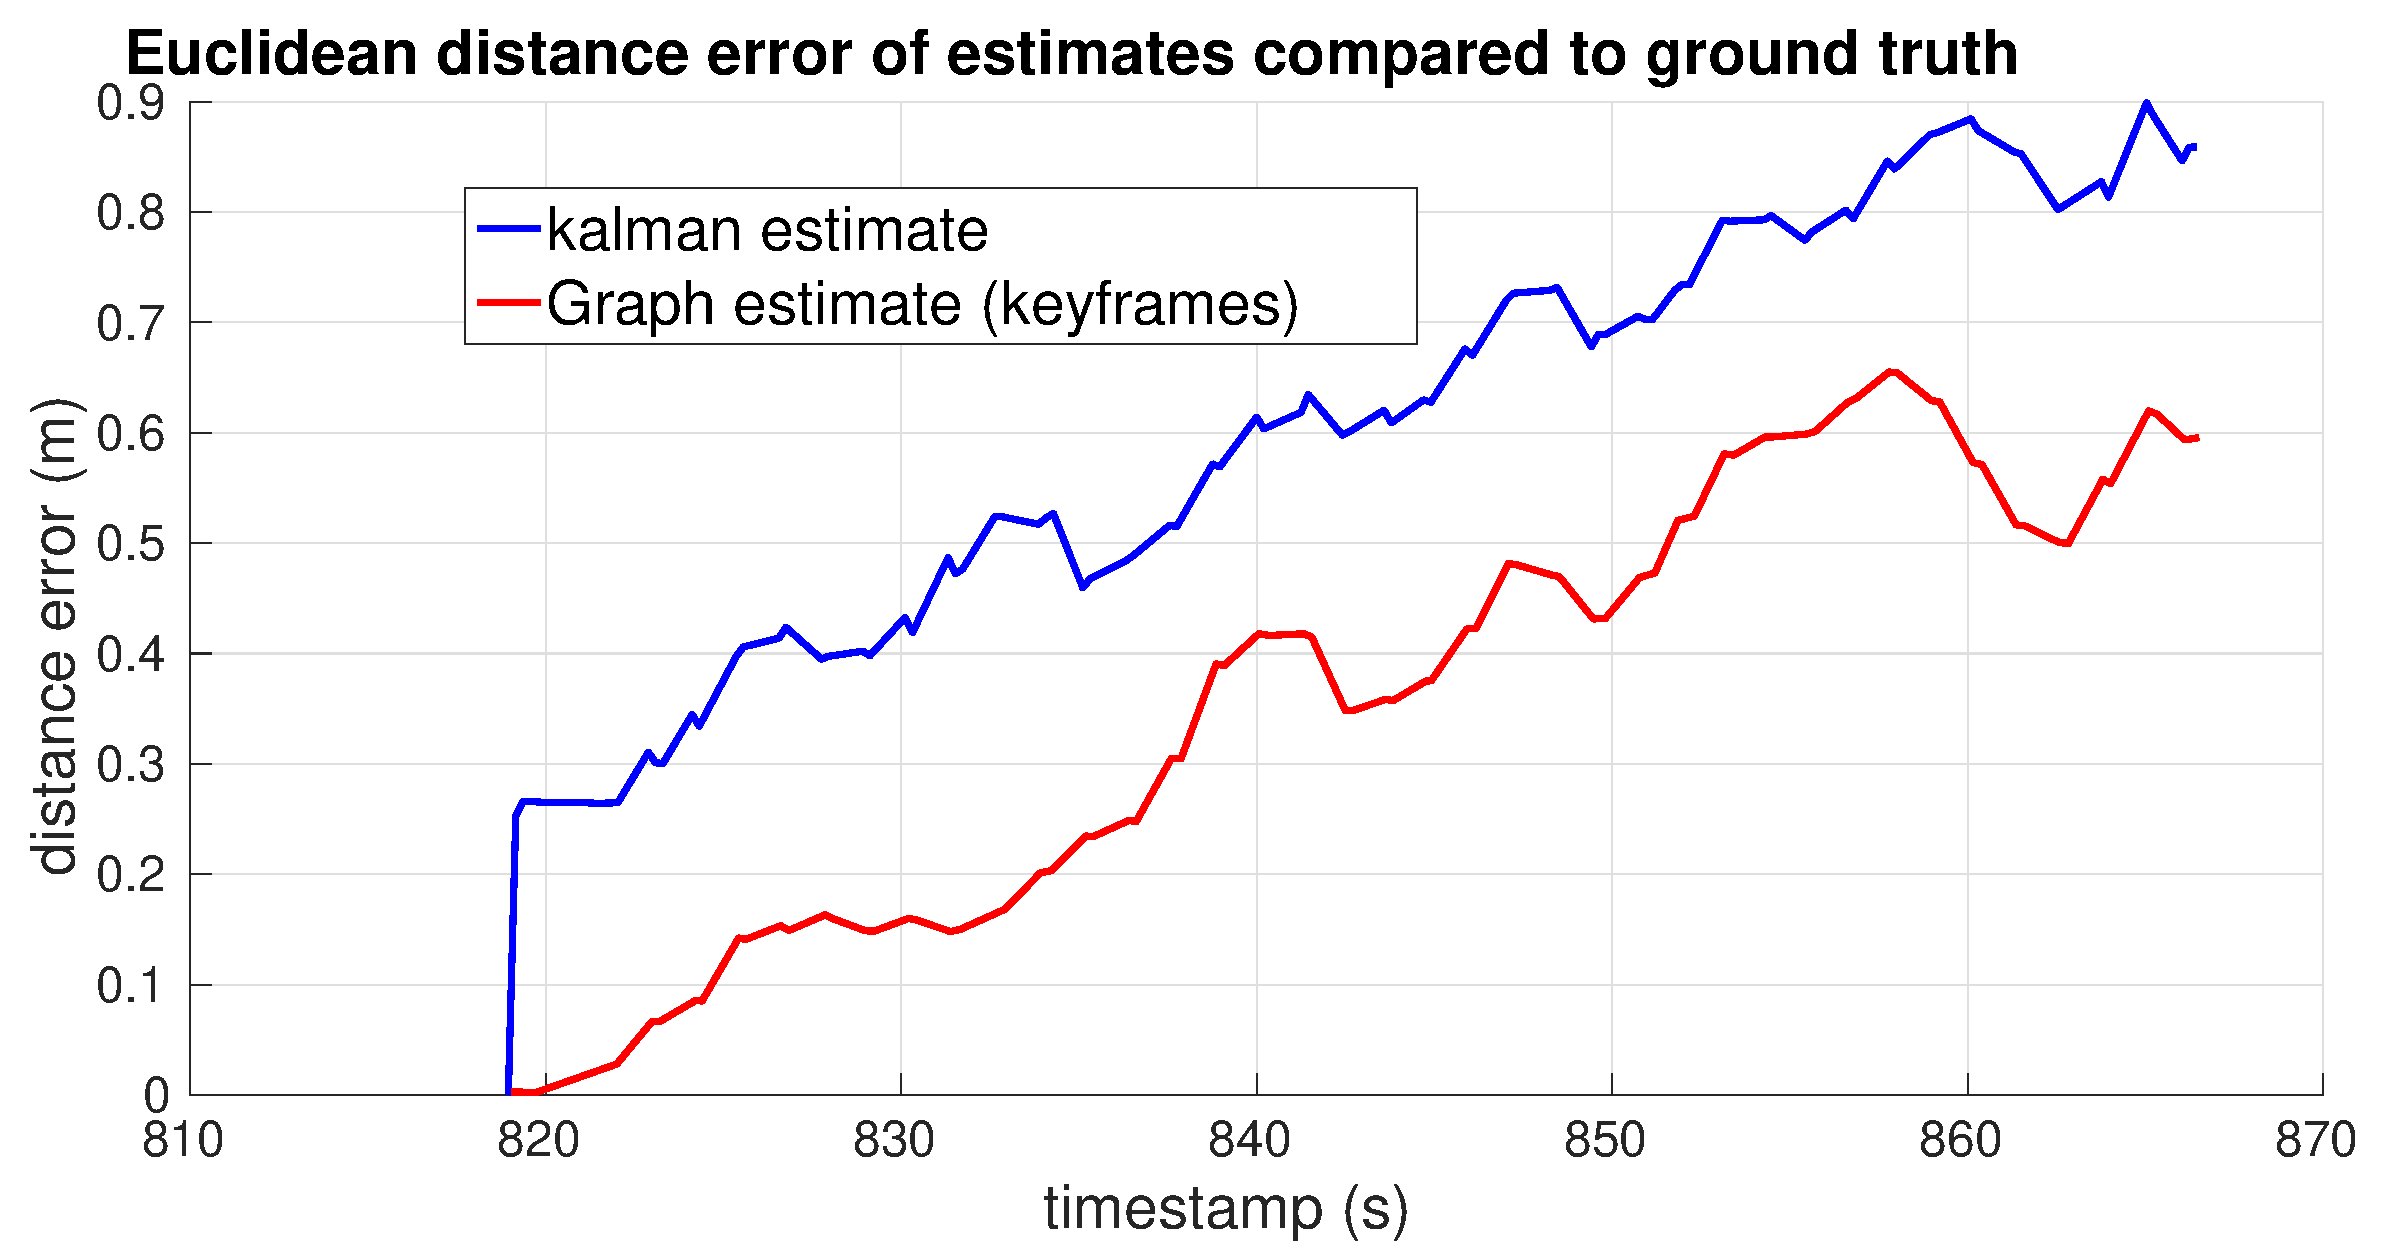
\includegraphics[scale=0.3]{figures/experiments/8shape/euclidean_err.eps}
\caption{ 
{\bf Top}: trajectory estimation during human 8-shaped walking phases with an IMU attached to a foot. Stars in blue and red colors are respectively the reference estimated states provided in the dataset and the estimation with our approach.
The continuous green line is the ground truth as given by the motion capture system.
{\bf Middle}: Evolution of estimated IMU biases and orientation of the device. Biases are estimated only for keyframes and considered as constant between them.
{\bf Bottom}: Evolution of euclidean distance errors between estimates and the ground truth for this 8-shaped walking trajectory.
}
\label{fig:8shape_walk}
\end{figure}

\begin{figure}[tb]
\centering
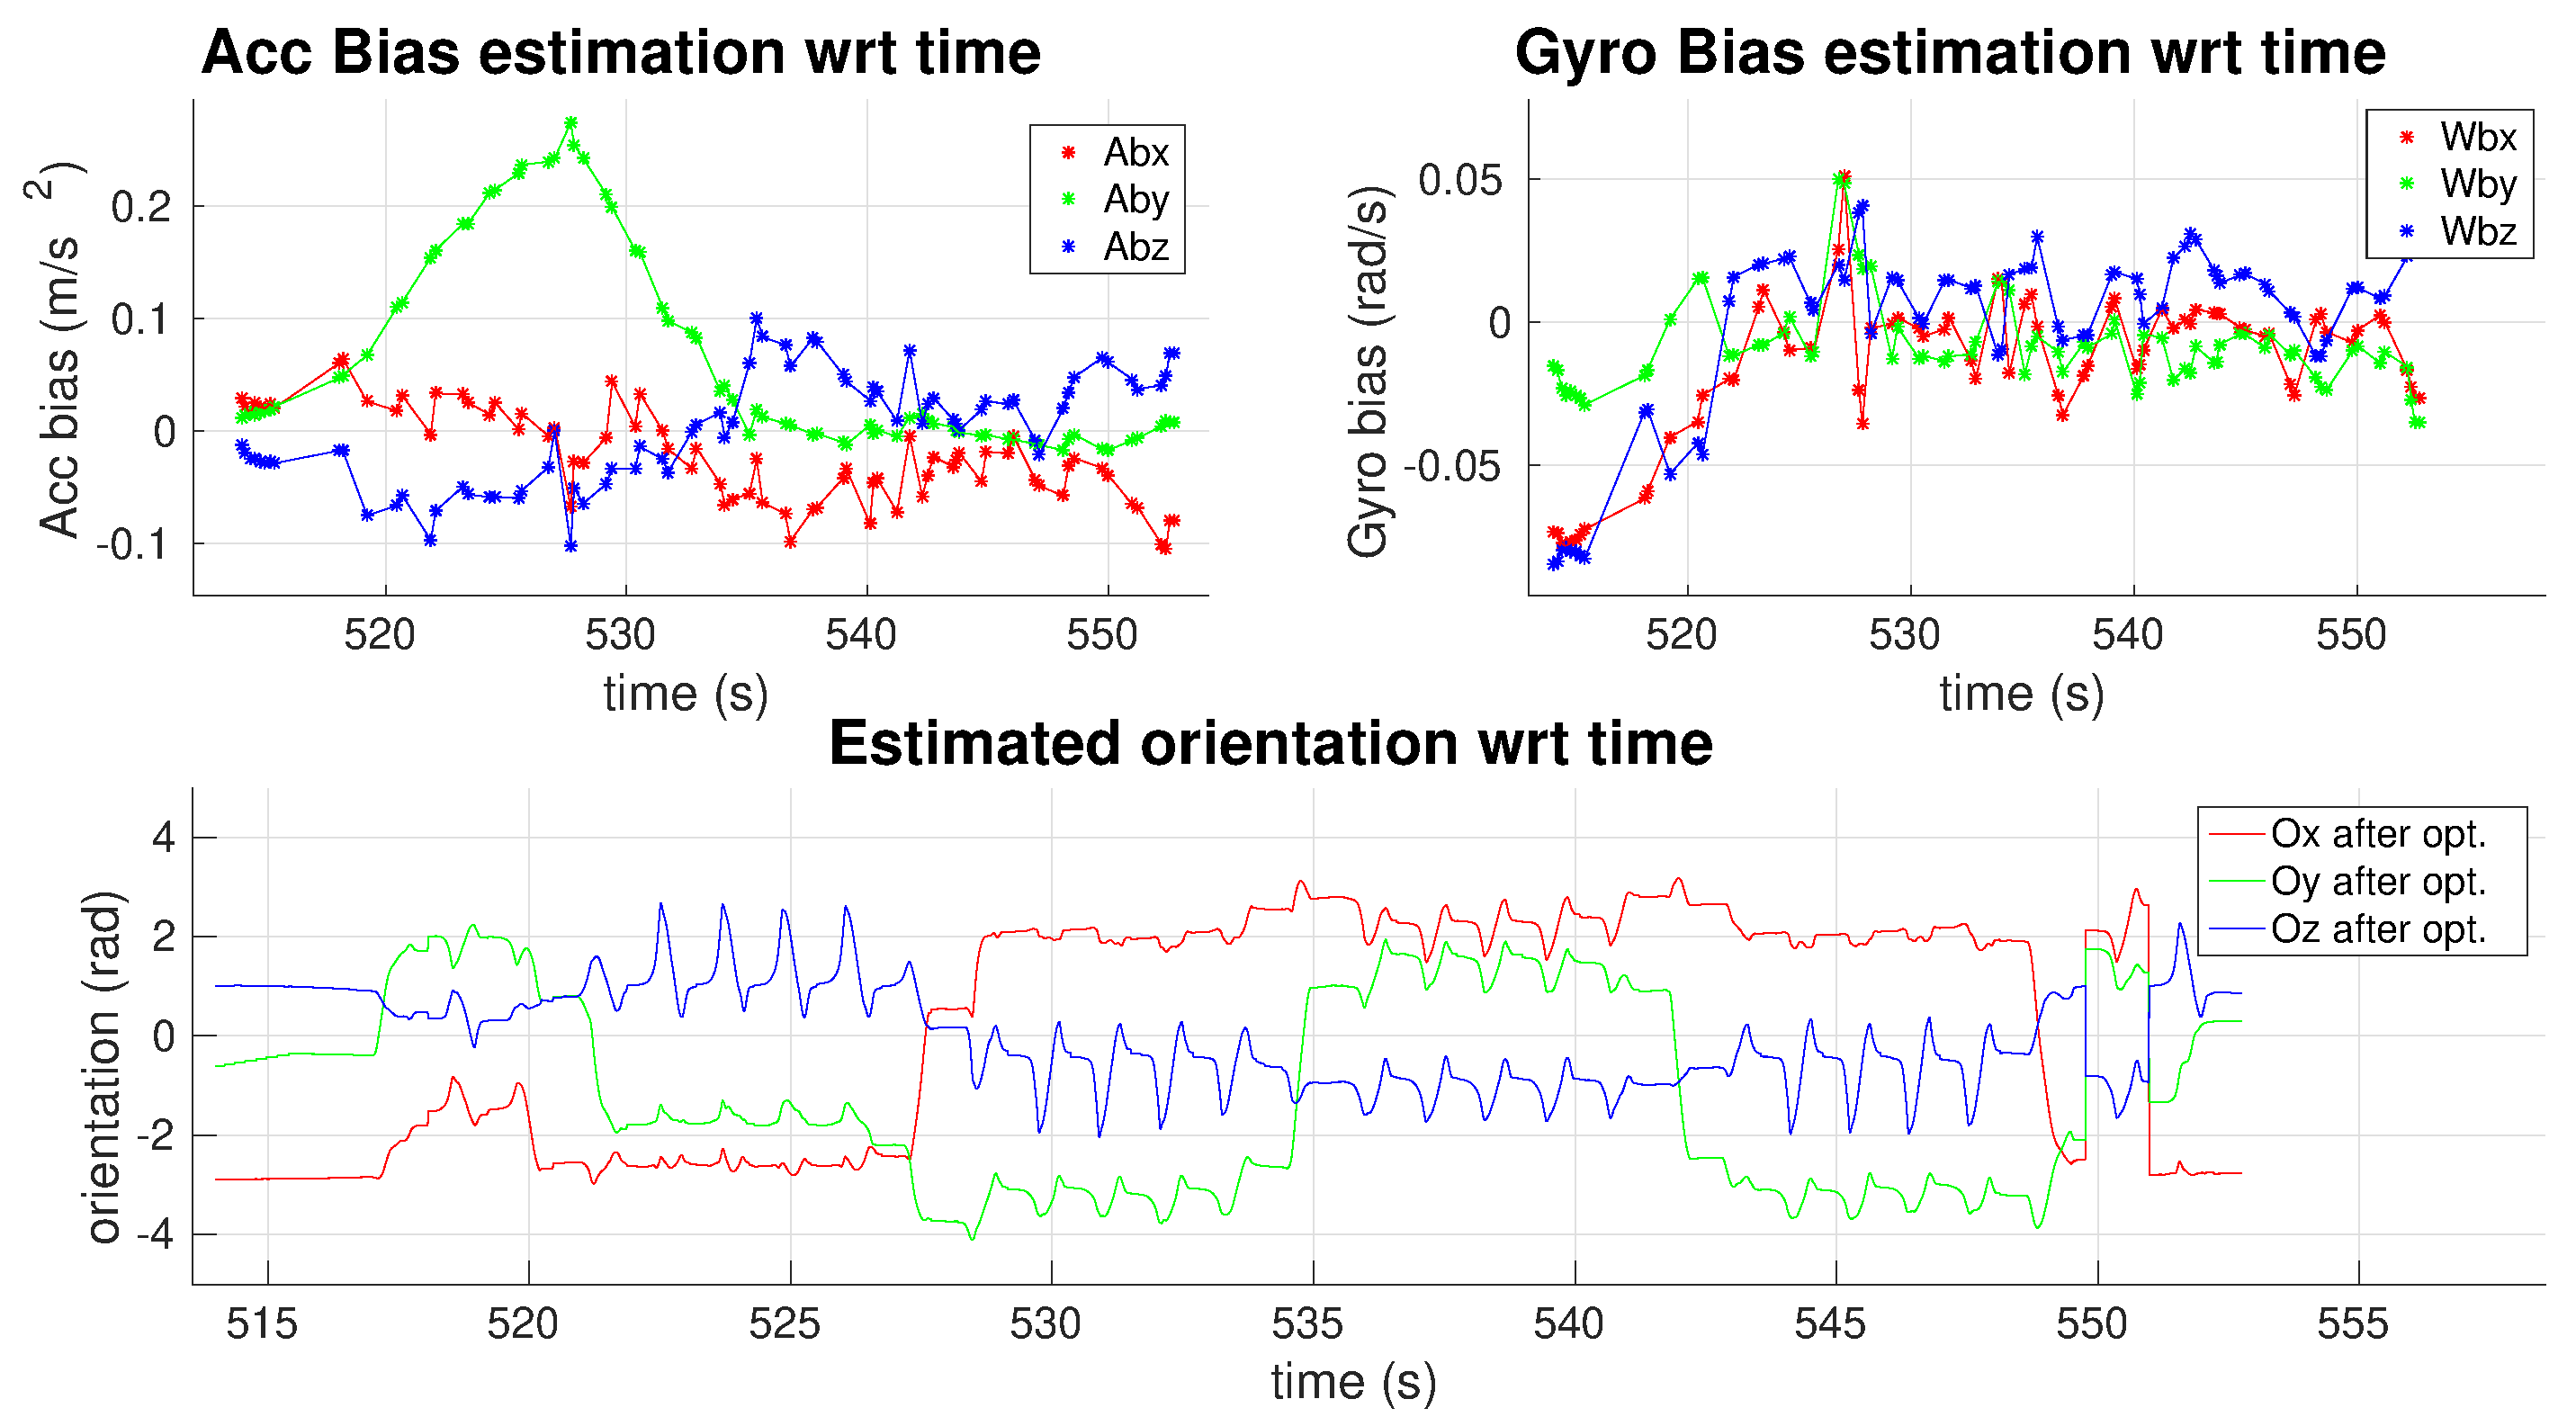
\includegraphics[scale=0.3]{figures/experiments/8shape/bias_orientation2.eps}
\caption{ 
Evolution of estimated IMU biases and orientation of the device during a curved walk. Biases are estimated only for keyframes and considered as constant between them.
}
\label{fig:curve_walk}
\end{figure}

% We fix the trajectory estimation problem by adding odometry information during foot's flying phase. However, we cannot fix any other conditions making velocity and bias observation possible hence all parameters of the state vector are estimated.
% This added KeyFrame reduces the integration time since last state optimization making bias random walk variation less critical on estimation. As we can see, results are much better and closer to MOCAP's ground truth as we could expect.



